% !TEX root = ./article.tex

\documentclass{article}

\usepackage{mystyle}
\usepackage{myvars}

\begin{document}

  \maketitle

  \section{Ejercicio 7}

    \paragraph{}
    El enunciado del ejercicio es el siguiente: \say{Se realiza un experimento para estudiar la efectividad de un nuevo tipo de somnífero, para lo cual se administra el mismo a 6 pacientes, mientras que a otros 6  se les da un somnífero estándar y a 6 más un placebo, durante una semana. En la tabla 6.33 se recogen las medias del número de  horas de sueño en las 7 noches para los 18 pacientes. (a=placebo, b= estándar, c=nuevo)}

    \paragraph{}
    Representamos los datos con un boxplot para observar su distribución de manera gráfica. Podemos ver que la distribución de Nuevo y Estandar parece similar, con Placebo teniendo horas de sueño por debajo de las otras dos.

    \paragraph{}
    Respecto a un análisis de las medias, obtendremos la comparación de ambos tipos de somnífero contra el control que ofrece el Placebo.


    \begin{figure}[h]
			\centering
      \begin{minted}{sas}
        proc anova;
          class TIPO;
          model HSUENYO=TIPO;
          means TIPO/dunnett('Placebo');
        run;
      \end{minted}
			\caption{}
			\label{code:sas_1}
		\end{figure}

    \paragraph{}
    proc anova nos proporciona de paso con el resultado del test de la hipótesis nula de que las medias de los tres grupos es igual, con un valor Pr > F 0.0003 podemos descartar esta hipótesis.

    \paragraph{}
    El test de dunnett ofrece intervalos de confianza para las diferencias de medias $\mu_{Placebo} - \mu_{i}$ siendo $i$ Estándar y Nuevo.

    \paragraph{}
    Los resultados de este test nos permiten rechazar la hipótesis de que cualquiera de los somníferos no tienen ningún efecto, ya que hay diferencias significativas entre ambos y el placebo a un nivel de confianza del 95%.

    \paragraph{}
    Sabiendo esto, realizamos un test de la T para comprobar si existen diferencias significativas entre las medias del somnífero estándar y del nuevo. Haremos esto mediante un contraste $L=0\mu{Placebo} + \mu_{Nuevo} - \mu_{Estándar}$. Si este contraste tiene valor 0, implica que las medias son iguales. Obtenemos además el estimador de $L$, que nos permite conocer, en caso de no ser 0, si L es positivo (el nuevo somnífero es mejor) o negativo (peor). clparm nos permite además obtener un intervalo de confianza para el estimador.

    \begin{figure}[h]
      \centering
      \begin{minted}{sas}
        proc glm;
          class TIPO;
          model HSUENYO=TIPO/clparm;
          contrast 'Eficacia de somnifero nuevo' TIPO -1 1 0;
          estimate 'Eficacia de somnifero nuevo' TIPO -1 1 0;
        run;
      \end{minted}
      \caption{}
      \label{code:sas_2}
    \end{figure}

    \paragraph{}
    El resultado del test sobre el contraste da un Pr > F del 0.7665, por lo que no podemos rechazar la hipótesis de que los dos somníferos tienen la misma eficacia. Por tanto, con un nivel de confianza del 95\% podemos afirmar que el nuevo somnífero no tiene un efecto significativo respecto a un somnífero estándar.

    \paragraph{}
    El estimador nos informa de que el somnífero nuevo produce 0.183 horas de sueño menos que el estándar, con un error de +/- 1.2921 horas. Esto coloca al efecto del nuevo somnífero entre 1.47 horas peor y 1.10 horas mejor que el estándar.

  \section{Ejercicio Acuicultura}

    \paragraph{}
    El enunciado del ejercicio es el siguiente: \say{Se quiere estudiar el efecto de distintas dosis de un medicamento para combatir a los parásitos de peces criados en acuicultura. Para ello, se tomaron 60 peces al azar, y se dividieron en 5 grupos de 12 individuos cada uno. El primer grupo no fue medicado, pero a los restantes se les suministró el medicamento en dosis crecientes. Tras una semana de tratamiento, se contabilizaron los parásitos existentes en cada individuo}.

    \paragraph{}
    Previamente, se ha realizado un preprocesado de los datos, que fueron suministrados de manera matricial, de tal manera que se tenía $5$ columnas cada una de ellas referidas a un tipo de tratamiento, junto con $12$ filas, cuyos valores en la celda se presuponen independientes entre si, referidas a las distintas observaciones de cada tratamiento. Por tanto, lo que se ha llevado a cabo es una transformación de dicha representación a una formada por $2$ columnas (grupo y niveles) y $60$ filas, donde cada una de ellas indica el tratamiento suministrado, junto con el nivel de parásitos obtenido.

    \subsection{Representa gráficamente los datos. ?`Te parece que el medicamento es efectivo contra los parásitos? Realiza un contraste de hipótesis para verificarlo.}

      \begin{figure}[h]
        \centering
        \begin{minted}{sas}
          proc boxplot data=peces_f;
            plot NIVELES*GRUPO;
          run;

          proc glm;
            class GRUPO;
            model NIVELES=GRUPO/clparm;
            contrast 'Eficacia medicamento' GRUPO 0.25 0.25 0.25 0.25 -1/e;
            estimate 'Eficacia medicamento' GRUPO 0.25 0.25 0.25 0.25 -1;
          run;
        \end{minted}
        \caption{}
        \label{code:sas_3}
      \end{figure}

      \paragraph{}
      Lo primero que se ha hecho es realizar una representación gráfica para conocer mejor la relación entre las variables. Por tanto, se ha elegido representar los datos mediante un \emph{Box Plot} que de la variable \texttt{niveles} particionada en los subgrupos determinados por el tipo de \texttt{grupo}.

      \begin{figure}[H]
        \centering
        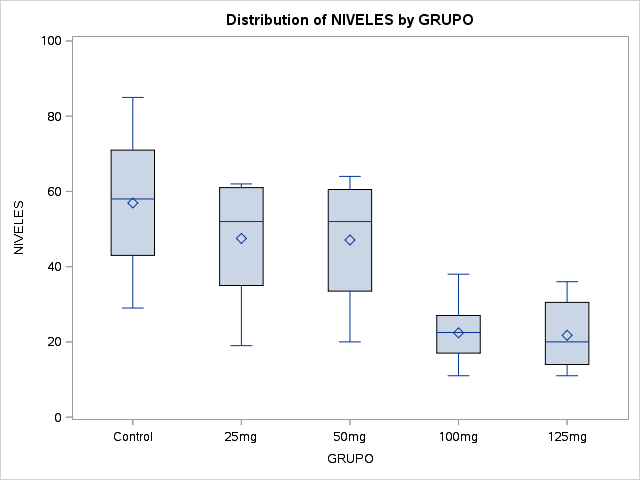
\includegraphics[width=0.7\textwidth]{boxplot1}
        \caption{Box Plot de la variable \texttt{niveles} condicionada por la variable \texttt{grupo}}
        \label{fig:figura_1}
      \end{figure}
      \paragraph{}

      \paragraph{}
      A partir de dicho gráfico se pueden apreciar dos grupos de medias diferentes, el primero de ellos formado por los tratamientos de \texttt{Control}, \texttt{25mg} y \texttt{50mg}, y el siguiente constituido por los tratamientos de \texttt{100mg} y \texttt{125mg}.

      \paragraph{}
      Para poder asegurar que el tratamiento es efectivo contra los parásitos se ha realizado el siguiente contraste de hipótesis:

      \begin{align}
        H_0:& \mu_{control} = \frac{\mu_{25mg} + \mu_{50mg} +\mu_{100mg} +\mu_{125mg}}{4} \\
        H_1:& \mu_{control} \neq \frac{\mu_{25mg} + \mu_{50mg} +\mu_{100mg} +\mu_{125mg}}{4}
      \end{align}

      \paragraph{}
      Si se acepta entonces podemos asegurar que el tratamiento no tiene efecto. Se ha escogido este contraste de hipótesis puesto que lo que se pretende comprobar es si el efecto del medicamento (en promedio) es diferente de los resultados que se obtienen sin el uso del mismo. Por tanto, se ha planteado como la igualdad de la media del valor de control y el promedio de las medias de cada cantidad de dosis del medicamento.

      \paragraph{}
      Dicho hipótesis se ha realizado con un nivel de confiaza del $95\%$, para la cual se ha obtenido un $\text{p-valor}\approx 0$. Por esta razón \textbf{tenemos que rechazar la hipótesis nula, lo que significa que el medicamento es efectivo}. Puesto que el estimador obtenido tiene signo negativo, es decir, que los distintos tratamientos disminuyen el nivel de parásitos con respecto del valor de control.

    \subsection{Obtén estimadores puntuales e intervalos de confianza para las medias de los tratamientos, utilizando dos métodos distintos, y explica las ventajas e inconvenientes de cada uno de ellos.}

    \begin{figure}[h]
      \centering
      \begin{minted}{sas}
        proc means clm;
          class GRUPO;
          var NIVELES;
        run;

        proc univariate cibasic;
          class GRUPO;
          var NIVELES;
        run;
      \end{minted}
      \caption{}
      \label{code:sas_4}
    \end{figure}

      \paragraph{}
      Para la obtención de los estimadores puntuales así como los intervalos de confianza se han utilizado los \emph{procs} \texttt{means} y \texttt{univariate} obteniendo los siguientes resultados en cada uno de ellos:


      \begin{figure}[H]
        \centering
        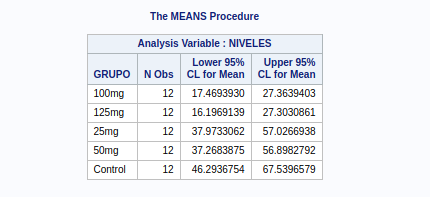
\includegraphics[width=0.7\textwidth]{EstimadoresMediasyIntervalos}
      \end{figure}

      \paragraph{}
      Estos dos métodos ofrecen los mismos resultados, sin embargo lo que les diferencia es la cantidad de información que aportan cada uno de ellos. En el caso de \texttt{means} la información es mucho más compacta y resumida, lo cual facilita su comprensión. Mientras que en el caso de \texttt{univariate} se obtiene información mucho más extendida y ampliada, como los valores de la varianza e intervalos de confianza para los estimadores de la esperanza y la varianza. Para casos en que se requiere de un resumen sencillo del conjunto de datos como es en este caso, es más apropiado el uso del \emph{proc} \texttt{means}

    \subsection{Analiza las diferencias significativas entre pares de medias de los 5 grupos utilizando diferentes métodos, comentando y comparando los resultados. ?`Cambian las conclusiones si utilizas $\alpha = 0.1$?}

      \begin{figure}[h]
        \centering
        \begin{minted}{sas}
          proc anova;
            class GRUPO;
            model NIVELES=GRUPO;
            means GRUPO/lsd duncan snk tukey bon scheffe lines alpha=0.1;
          run;
        \end{minted}
        \caption{}
        \label{code:sas_5}
      \end{figure}

      \paragraph{}
      Para la realización de los distintos tests se han utilizando los siguientes métodos: \emph{Método de la T}, \emph{Duncan}, \emph{Newman–Keuls}, \emph{Tukey}, \emph{Bonferroni} y \emph{Schefeé}. Estos se dividen en dos grupos, los que aseguran los resultados para experimentos múltiples con una confianza global de $1-\alpha$(\emph{Newman–Keuls}, \emph{Tukey}, \emph{Bonferroni} y \emph{Schefeé}) y los que no aseguran dicho nivel de confianza (\emph{Método de la T}, \emph{Duncan}).

      \paragraph{}
      Se ha probado con un valor $\alpha = 0.05$, para el cual se han obtenido los mismos resultados en todos los tests: Existen dos grupos de medias, el formado por \texttt{Control}, \texttt{25mg} y \texttt{50mg}, y el siguiente constituido por los tratamientos de \texttt{100mg} y \texttt{125mg} tal y como se podía intuir en el gráfico de la figura \label{fig:figura_1}.

      Después se ha realizado el mismo conjunto de tests con $\alpha = 0.1$ obteniendo los mismos resultados que para el caso anterior en los tests que aseguran un nivel de confianza global $1-\alpha$, mientras que en el resto (\emph{Método de la T}, \emph{Duncan}), estos indican que la media del grupo \texttt{Control} es diferente del grupo formado por los tratamientos \texttt{25mg} y \texttt{50mg}, por lo que afirman la existencia de 3 grupos de medias diferentes.

    \subsection{Realiza el test de Dunnett para comparar los efectos de las distintas dosis con el grupo \texttt{control} y comenta el resultado.}

      \begin{figure}[h]
        \centering
        \begin{minted}{sas}
          proc anova;
            class GRUPO;
            model NIVELES=GRUPO;
            means GRUPO/dunnett('Control');
          run;
        \end{minted}
        \caption{}
        \label{code:sas_6}
      \end{figure}

      \paragraph{}
      Tras aplicar el test de \emph{Dunnett} usando el tratamiento \texttt{control} para compararlo con el resto de tratamientos con un nivel de confianza de $\alpha=0.05$ para todo el experimento, se ha concluido que las medias de los tratamientos \texttt{100mg} y \texttt{125mg} son diferentes de las de \texttt{control}. Sin embargo, las de \texttt{25mg} y \texttt{50mg} son tomadas como iguales.


    \subsection{Se desea comparar el efecto de las dosis bajas del medicamento, \texttt{25-50 mg} con el de las dosis altas, \texttt{100-125 mg}. Construye un intervalo de confianza para la diferencia entre ambos efectos e interpreta el resultado obtenido}

      \begin{figure}[h]
        \centering
        \begin{minted}{sas}
          proc glm;
            class GRUPO;
            model NIVELES=GRUPO/clparm;* se obtiene I.C. para el contraste pedido;
            contrast 'dosis bajas contra dosis altas' GRUPO .5 .5 -.5 -.5 0/e;
            estimate 'dosis bajas contra dosis altas' GRUPO .5 .5 -.5 -.5 0;
          run;
        \end{minted}
        \caption{}
        \label{code:sas_7}
      \end{figure}

      \paragraph{}
      En este caso se ha planteado el contraste de hipótesis como la igualdad del promedio de medias de dosis altas con las dosis bajas, por tanto puede escribirse como:

      \begin{align}
        H_0:& \frac{\mu_{25mg} + \mu_{50mg}}{2} = \frac{\mu_{100mg} +\mu_{125mg}}{2} \\
        H_1:& \frac{\mu_{25mg} + \mu_{50mg}}{2} \neq \frac{\mu_{100mg} +\mu_{125mg}}{2}
      \end{align}

      \paragraph{}
      Se ha realizado dicho contraste con un nivel de confianza $1-\alpha$ con $\alpha = 0.05 $, para el cual se obtiene un $\text{p-valor}\approx 0$ por lo que se debe rechazar la hipótesis nula, es decir, no existe igualdad de medias entre los resultados obtenidos con dosis bajas y dosis altas.

      \paragraph{}
      El intervalo de confianza para el estimador de la diferencia de medias obtenido es $[-32.88, -17.53]$. Esto puede interpretarse como que las dosis altas disminuyen el nivel de parásitos entre $17.53$ y $32.88$ respecto de las dosis bajas.

    \subsection{Verifica las hipótesis del modelo con ayuda de gráficos de residuos}

      \begin{figure}[h]
        \centering
        \begin{minted}{sas}
          proc anova;
            class grupo;
            model niveles=grupo;
            means grupo/hovtest ;
          run;

          proc glm;
            class grupo;
            model niveles=grupo;
            output out= resal p=pred r=res student=rst;
            proc print data=resal;
          run;

          proc univariate plot normal data=resal;
            var res;
          run;
        \end{minted}
        \caption{}
        \label{code:sas_8}
      \end{figure}

      \paragraph{}
      Para verificar la hipótesis del modelo se han realizado distintas pruebas, entre ellas se ha estudiado la hipótesis de igualdad de varianzas entre los distintos tratamientos. También se ha analizado la distribución de los residuos obtenidos, para comprobar que sigue una distribución normal.

      \paragraph{}
      En el caso de la hipótesis de igualdad de varianzas, esta se llevado a cabo a partir del test de \emph{Levene} para el cual se ha obtenido un $\text{p-valor} \approx 0.027$. Por tanto, a un nivel de confianza del $95\%$ tendríamos que rechazar la hipótesis de que las varianzas son iguales. Sin embargo dicha hipótesis se puede aceptar si se toma un nivel de confianza del $98\%$.

      \paragraph{}
      En cuanto a la hipótesis de normalidad de la distribución de residuos, se puede admitir que esta es cierta debido a los resultados obtenidos en los distintos tests de normalidad. Esta idea se refleja en el gráfico de normalidad de los residuos, el cual se muestra en la figura \ref{fig:figura_2}.

      \begin{figure}[H]
        \centering
        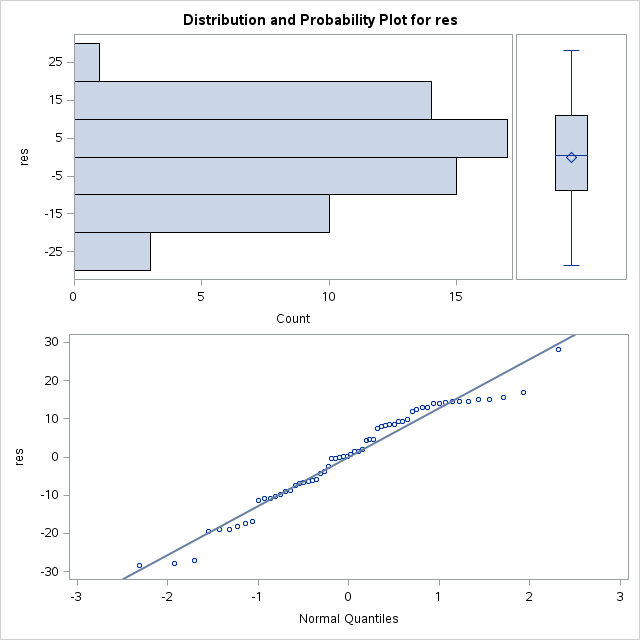
\includegraphics[width=0.7\textwidth]{Normalidadresiduos7}
        \caption{Gráfico de normalidad de residuos}
        \label{fig:figura_2}
      \end{figure}



    \subsection{Suponiendo que los grupos de datos correspondieran a cinco medicamentos elegidos aleatoriamente entre todos los posibles en el mercado, ?`cómo cambiaría el modelo adecuado? ?`Podría afirmarse que existe variación significativa entre los efectos de los distintos medicamentos? Estima las componentes de la varianza bajo dicho supuesto}


      \begin{figure}[h]
        \centering
        \begin{minted}{sas}
          proc glm;
            class grupo;
            model niveles=grupo;
            random grupo/test;
          run;
        \end{minted}
        \caption{}
        \label{code:sas_8}
      \end{figure}

      \paragraph{}
      En este caso, en lugar de plantear el problema como un análisis de la varianza (ANOVA) de un factor con $k$ tratamientos distintos, lo deberemos plantear como un análisis de la varianza desde el punto de vista de un factor aleatorio. De esta manera, el conjunto de pasos a realizar para llevar a cabo el test de hipótesis no varía. Sin embargo la interpretación es distinta, ya que ahora en lugar de estudiar si existen tratamientos diferentes entre si y sus diferencias, el problema se plantea como conocer si todos los niveles extraidos como muestra pertenecen a una misma población.

      \paragraph{}
      Al igual que se concluyó en anteriores apartados, en este caso también hay que rechazar la hipótesis nula, debido a que el $\text{p-valor}$ toma un valor extremadamente bajo $\text{p-valor}\approx 0$. Puesto que hemos rechazado la hipótesis nula, podemos estimar el valor de la varianza entre los niveles tal y como se indica a continuación:

      \begin{align}
        Var(Error) + 12 Var(GRUPO) &= 3093.23\\
        Var(Error) &= 176 \\
        &\implies Var(GRUPO) = \frac{3093.23 - 176}{12} = 243.1025
      \end{align}


\end{document}
